
%(BEGIN_QUESTION)
% Copyright 2006, Tony R. Kuphaldt, released under the Creative Commons Attribution License (v 1.0)
% This means you may do almost anything with this work of mine, so long as you give me proper credit

Her vises et skjemadiagram for en enkel, analog, kun-proporsjonal regulator:

$$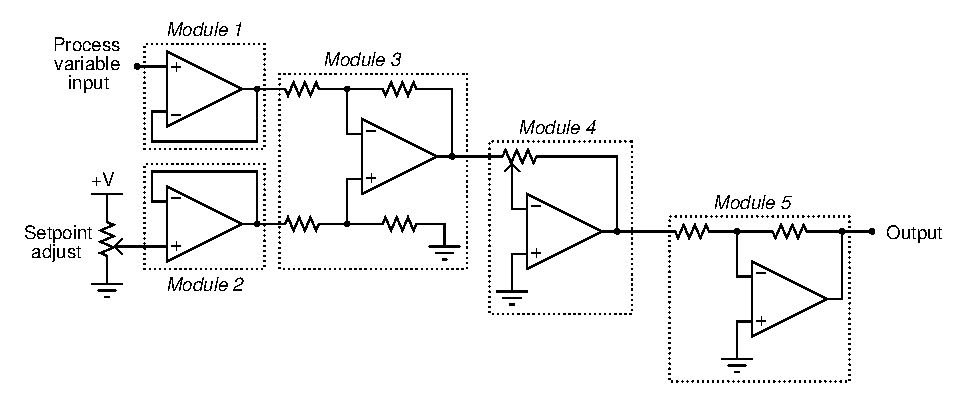
\includegraphics[width=15.5cm]{i01534x01.eps}$$

Forklar hva du måtte gjøre for å øke proporsjonalbåndet i denne regulatorkretsen, og avgjør også om den er {\it direktevirkende} eller {\it reversvirkende}.

\vskip 10pt

Vurder nå denne modifikasjonen av regulatorkretsen, som gir både {\it proporsjonal} og {\it deriverende} regulering, ofte omtalt som P+D eller PD-regulering:

$$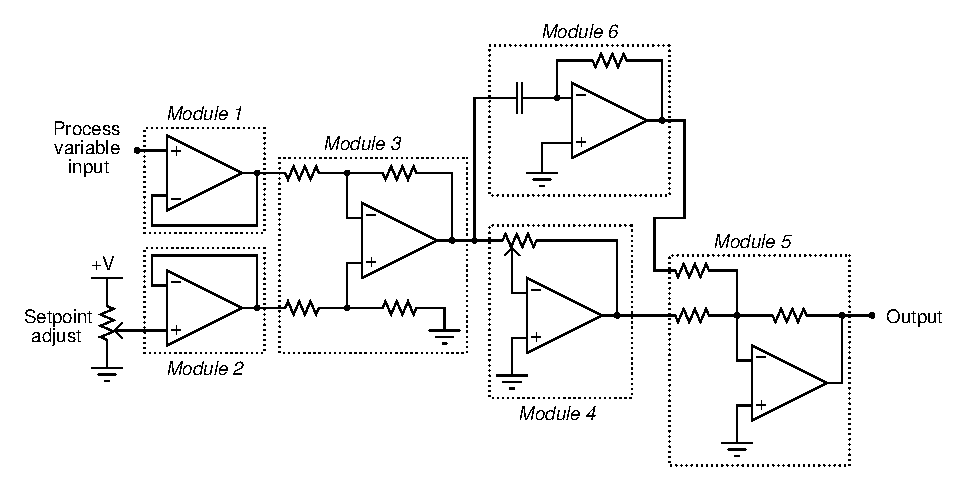
\includegraphics[width=15.5cm]{i01534x02.eps}$$

Forklar hvordan den ekstra modulen (Modul 6) implementerer deriverende regulering, og hva som må endres i kretsen for å øke $\tau_d$ (dvs. gjøre den deriverende virkningen mer aggressiv).

\underbar{file i01534}
%(END_QUESTION)





%(BEGIN_ANSWER)

For å øke proporsjonalbåndet (redusere forsterkningen), flytt glideren på potensiometeret mot høyre (Modul 4). Dette er en {\it reversvirkende} regulator.

\vskip 10pt

For å øke aggressiviteten i den deriverende virkningen, øk kondensatorverdien (Modul 6) og/eller reduser verdien på summeringsmotstanden i Modul 5 som tar imot utgangssignalet fra Modul 6.

%(END_ANSWER)





%(BEGIN_NOTES)

For å øke aggressiviteten i den deriverende virkningen, øk kondensatorverdien (Modul 6) og/eller reduser verdien på summeringsmotstanden i Modul 5 som tar imot utgangssignalet fra Modul 6.

%INDEX% Control, derivative: analog electronic controller

%(END_NOTES)
